\documentclass[12pt]{report}
\usepackage[french]{babel}
\usepackage[utf8x]{inputenc}
\usepackage{graphicx}
\usepackage{dsfont}
\usepackage{amsfonts}
\usepackage{svg}
\usepackage[T1]{fontenc}
\usepackage{listings}
\usepackage{minted}
\newcommand{\deriv}{\mathrm{d}}

\begin{document}

\begin{titlepage}

\newcommand{\HRule}{\rule{\linewidth}{0.5mm}} % Defines a new command for the horizontal lines, change thickness here

\center 

\textsc{\LARGE Compte rendu Programmation 3D}\\[1.5cm]
\textsc{\Large Open GL et PBR}\\[0.5cm] 
%\textsc{\large SE331}\\[0.5cm] 


\begin{minipage}{0.4\textwidth}
\begin{flushleft} \large
\center
Ludovic \textsc{LONLAS}\\ % Your name
\end{flushleft}

\end{minipage}\\[2cm]

{\large \today}\\[2cm]


\includegraphics[width=1.5cm]{Logo_FDS_Quadri_Grand_2392x2950-243x300.png}

\includegraphics[width=1.5cm]{LOGO_RVB_grand-UM.jpg}\\[1cm]
\end{titlepage}



J'ai eu énormément de difficultés à réalisé ce TP, il s'avère qu'il n'existe pas énormément de documentation pour OpenGL, de plus pour implémenter du code dans le squelette du cour, j'ai du adapté les algorithmes pour qu'ils marchent.

Charger une texture depuis un fichier et la plaquer contre un mesh n'a pas été très dur, charger une deuxième texture dans le fragment shader à pris plus de temps mais il fallait juste les bind à des textures actives différentes.
\\\\
La skybox,
malgré le code fourni dans le cour et sur LeanOpenGL.com j'ai eu énormément de mal à la  faire marché, dans un premier temps mon cube n'afficher qu'une face, ensuite les textures ne voulaient pas se charger dans le shader, après avoir résolu ces problèmes, je me suis retrouvé bloqué car quand j'affichais mon mesh, la skybox disparaissait, la raison qui n'était pas évidente car il n'y avait pas de messages d'erreur était que je ne mettais en mémoire les sommets qu'une fois.
Une fois ces problèmes résolues j'ai réussi à implémenté le shader miroir en quelques minutes.



\begin{figure}[h!]
    \centering
    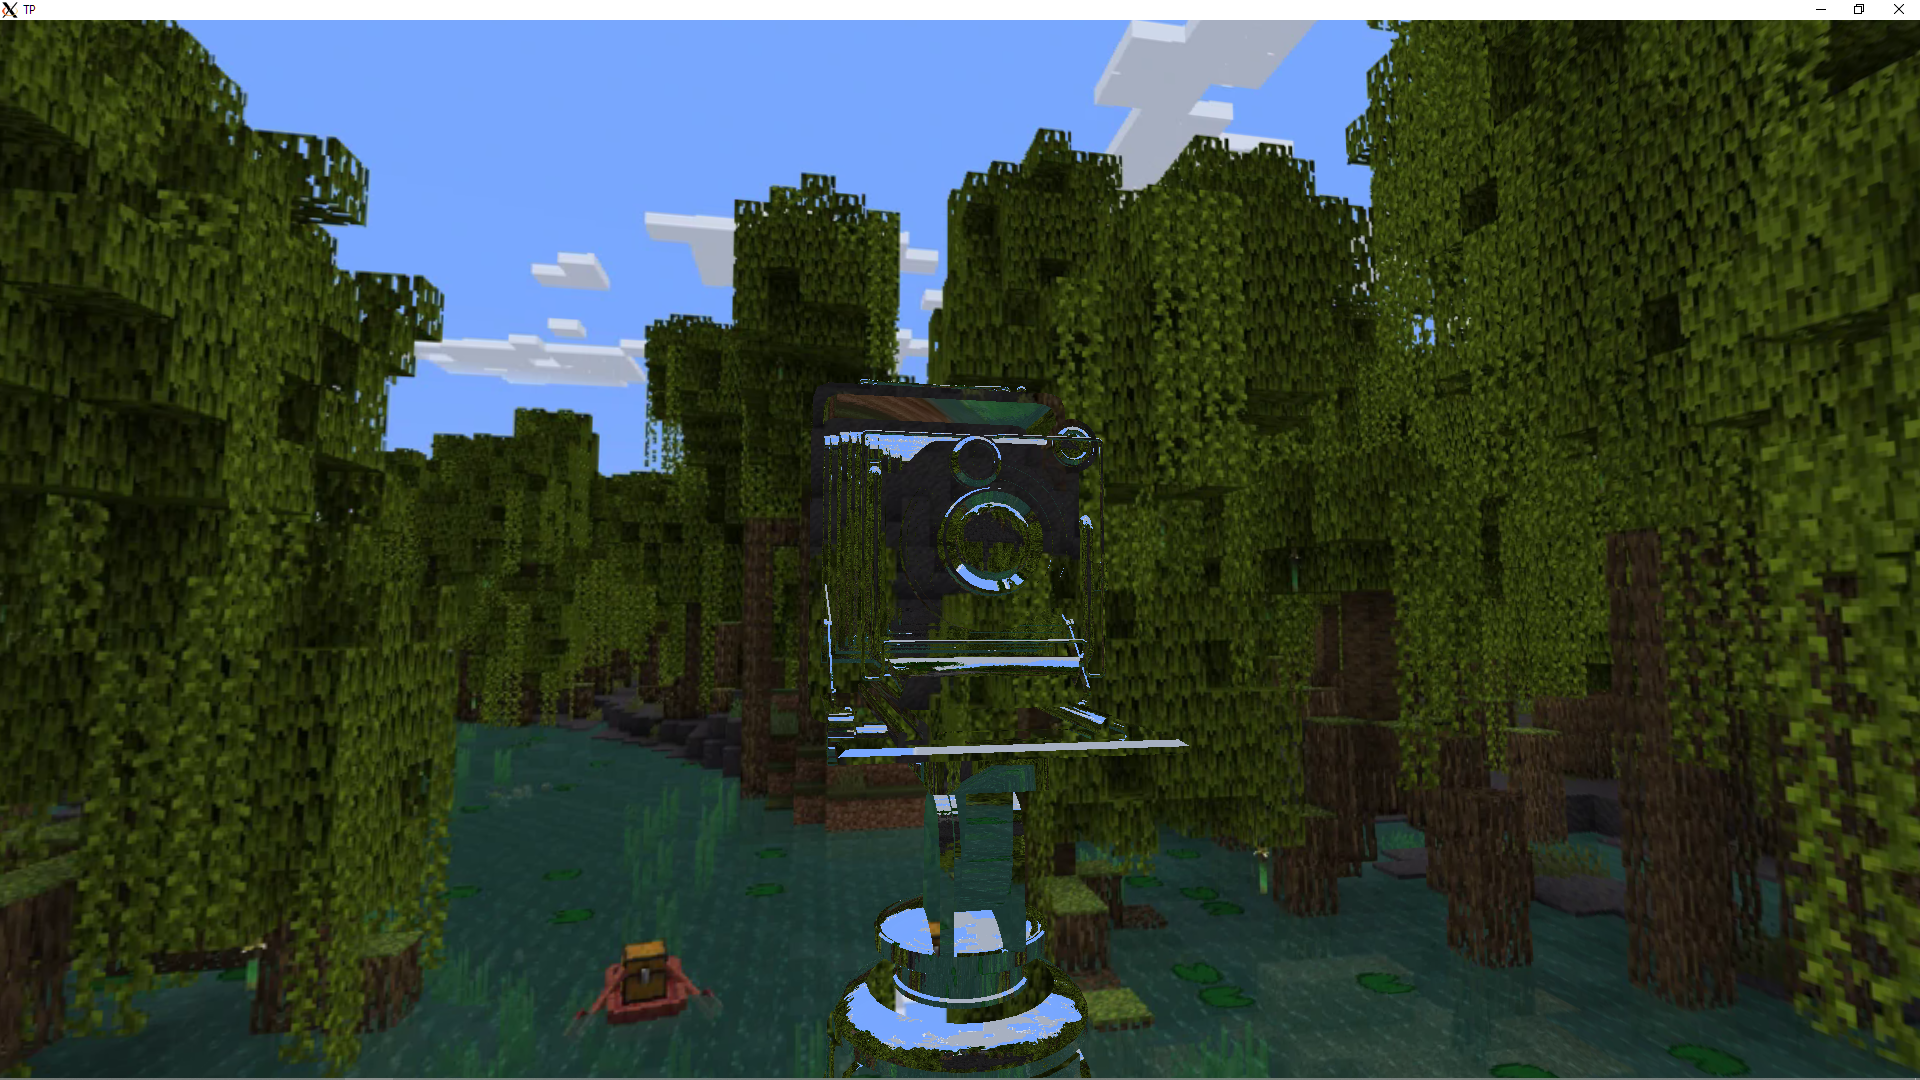
\includegraphics[width=12.0cm]{minecraft2.png}
    \caption{Rendu mirroir de Antique\_Camera.gltf}
    \label{fig:1}
\end{figure}

\newpage
Seconde partie du TP,
\\
Je n'ai pas réussi cette partie du TP, je peux charger la texture de base, la normal map, la metalness et la roughness d'un modèle 3D, je les utilisent tous dans un shader sauf pour la roughness.\\ J'ai passé plus de 10 heures à essayer de flouter la cubemap ainsi que d'autres méthodes mais je n'ai pas réussi à en faire marché une seule, j'ai essayé de créer une mipmap, pour ensuite chargé des textures de plus basses résolutions mais ça n'a pas marché, j'ai aussi voulu implémenter le rendu PBR mais sans succès.\\
\begin{figure}[h!]
    \centering
    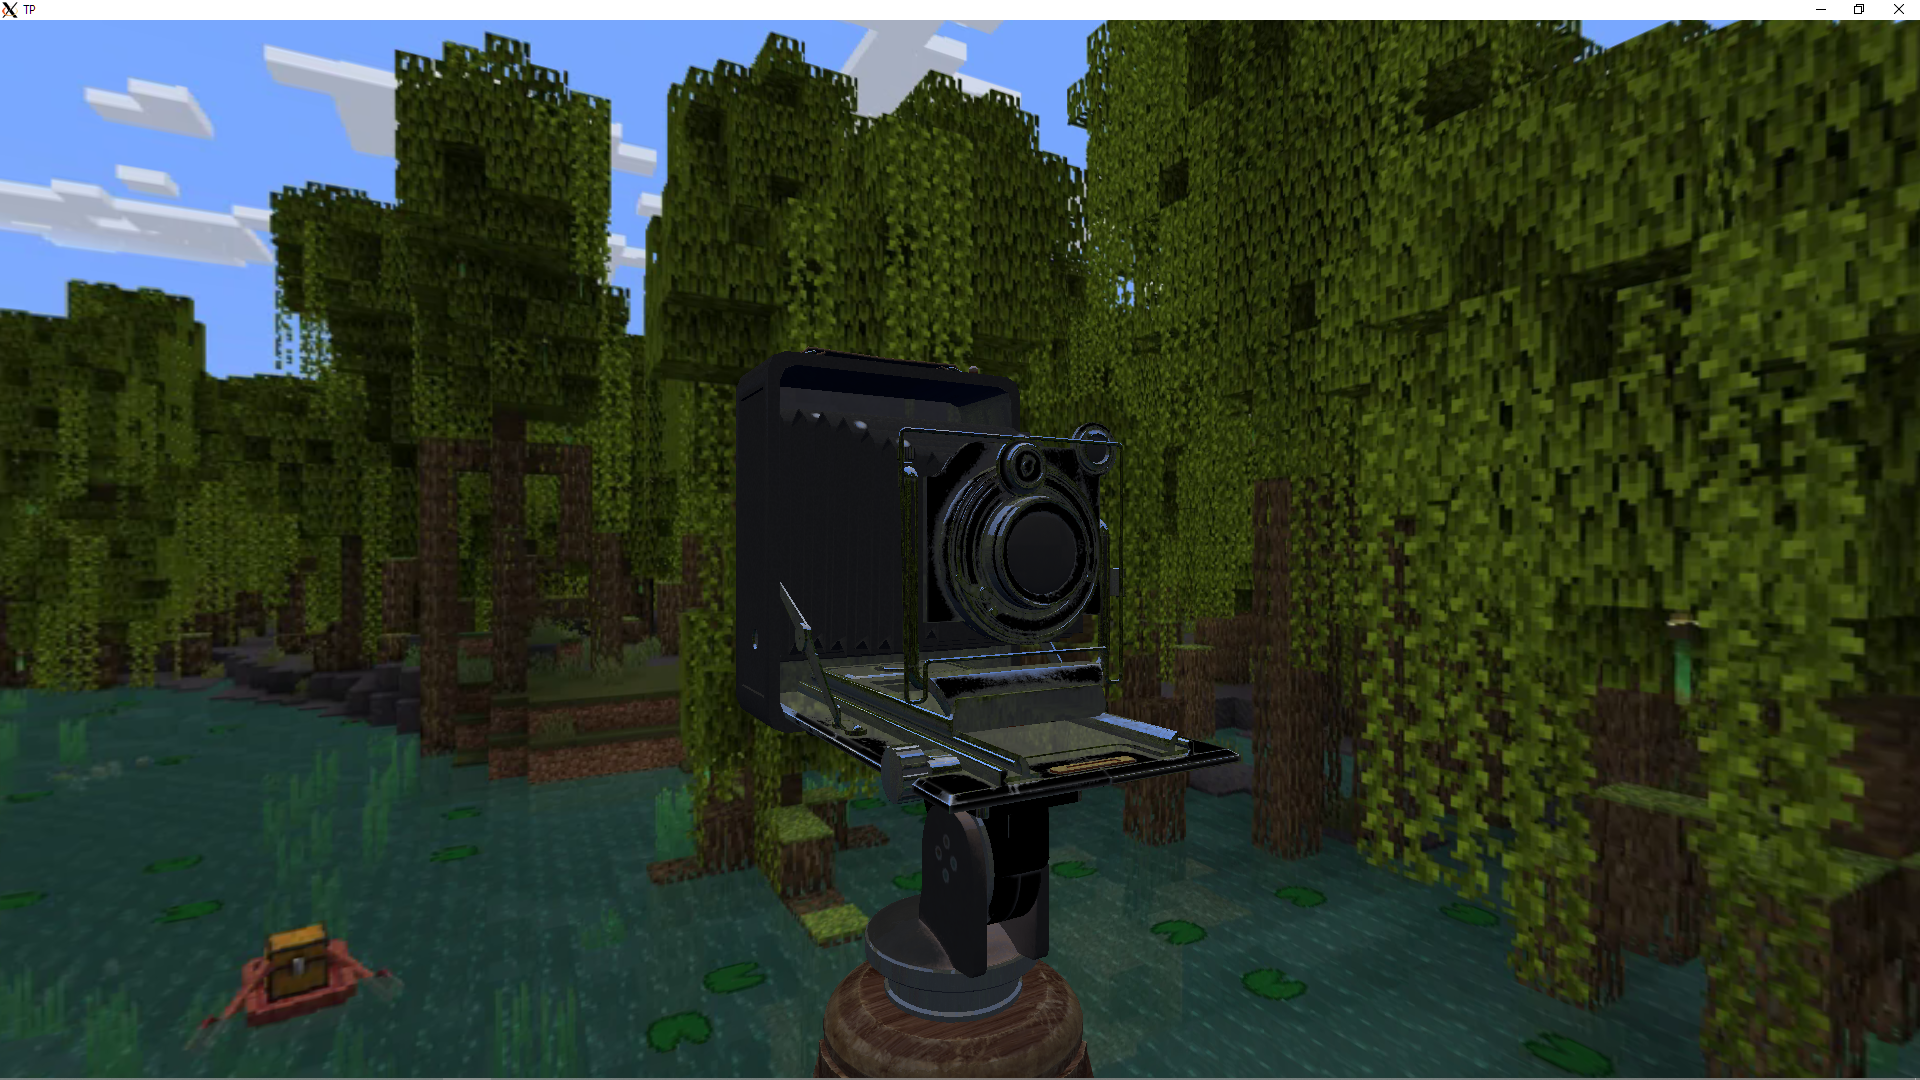
\includegraphics[width=12.0cm]{minecraft.png}
    \caption{Rendu de Antique\_Camera.gltf avec mon shader}
    \label{fig:1}
\end{figure}
\\
J'aurais bien aimé, rajouté l'effet d'émission mais je n'ai plus assez de temps pour le faire.\\
J'ai compris que pour le réalisé il aurais fallu créer une carte de luminance pour chaque modèle en projetant les matériaux émissif sur les faces d'un cube. Je ne sais pas comment implémenter un effet d'occlusion ambiante.\\
\\
Je regrette ne pas avoir pu finir ce TP, pour la plupart des problèmes que j'ai rencontrer j'ai pris énormément de temps à les résoudre car il est très dur de trouver la cause du problème, et car les aides en ligne sont limité à principalement vos cours(merci) et à LearnOpenGL.com , la documentation des fonctions d'OpenGL quand elle existe ne m'a pas aidé durant ce TP. 


\end{document}